\section{Study Design}\label{sec:studyDesign}

\subsection{Study overview}

The study connects an occurrence-level detector evaluation to a repository-level description of detector output. We first identified open-source Java repositories that use jOOQ and retain generated schema classes. We then annotated a size-stratified sample, partitioned its projects into training, validation, and test sets, selected one detector configuration on the validation set, and evaluated it on the held-out test set. Finally, we applied the selected detector to the full identified corpus and coded recurring source-fragment patterns among two classes of flags.

Reference and predicted occurrences are class-labelled line spans within files, which the held-out evaluation matches one to one. The corpus analysis counts detector flags and repositories with at least one flag.

\subsection{Repository mining and target population}\label{sec:mining}

The target population comprises repositories identified by our dated GitHub search and subsequent filters. We required Java code that used jOOQ for database access and jOOQ-generated classes stored in version control \nobreakcite{jooq2025code}. These classes expose database objects such as tables, columns, and constraints to source analysis.

On 10 January 2026, we queried the GitHub Code Search application programming interface (API) \nobreakcite{githubSearchApi} for jOOQ dependency declarations in project manifests. The API returned at most \num{1000} results for each search. Searching Java import statements could return many files from the same large repository, allowing duplicate repository hits to occupy much of that limit. We instead searched dependency declarations in Maven and Gradle manifest formats \nobreakcite{maven2026homepage,gradle2026homepage}, such as \texttt{pom.xml}, \texttt{build.gradle}, and \texttt{build.gradle.kts}. A project generally has far fewer manifest files than Java source files, so this choice was intended to reduce duplicate saturation and admit more distinct repositories within each result cap.

We made each manifest query specific enough to remain below the limit where possible. Queries with more than \num{1000} matches yielded only the \num{1000} results most recently indexed by GitHub. The search could also miss repositories that used another build system or expressed their dependency in a form absent from our queries. Online Resource~1 provides the exact search terms and omitted-project list. All later repository counts refer to this identified population.

The search returned \num{3829} repositories. We retained \num{802} that stored jOOQ-generated classes in version control. We then required at least one Java file that was not generated and that referenced jOOQ or a generated class. This filter established that the repository contained application source using the representation under study in addition to generated artefacts. It also excluded repositories whose relevant application code used another language on the Java Virtual Machine. The content filter left \num{645} repositories.

Finally, we reviewed the remaining repositories for copies that could cross project partitions or receive repeated weight in the corpus counts. Google Gemini 3 Pro Preview \nobreakcite{gemini3ProPreview} screened the \num{645} repository file trees and proposed duplicate candidates. We manually reviewed every proposal before omitting a repository. This process removed \num{42} duplicates or unsuitable copies and yielded the preliminary \num{603}-repository corpus used for sampling. A further duplicate found before corpus execution reduced the final analysis corpus to \num{602} repositories. Figure~\ref{fig:dataFunnel} records these successive boundaries.

\begin{figure}[tbp]
    \centering
    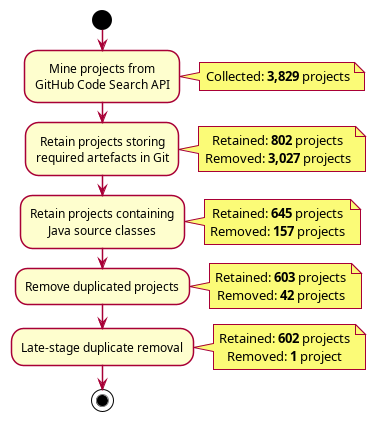
\includegraphics[width=200pt]{figures/data_funnel_diagram.png}
    \caption{Repository selection for the study. A GitHub manifest search on 10 January 2026 returned \num{3829} repositories; source-content filters and duplicate review produced a preliminary corpus of \num{603} repositories and a final corpus of \num{602}. The resulting corpus is the study's identified target population.}
    \label{fig:dataFunnel}
\end{figure}

This mining procedure establishes the population to which the corpus counts refer. The next step defines which files and antipattern occurrences the study measures within that population.

\subsection{Operational scope}\label{sec:antipatternSelection}

We studied static evidence available in Java source code. A relevant file was either generated by jOOQ or contained a reference to jOOQ or a generated class. The first group carried database-design evidence. The second group identified source that directly constructed queries or used generated database objects. This definition excluded Java files with no observable connection to the analysed database-access representation.

A manually maintained path list removed generated files that did not contribute evidence for antipattern detection, including records and plain data objects. It also removed classes generated from database entities outside the application, such as system schemas and tables managed by database extensions. These exclusions kept repository size and annotation effort tied to source that could contain an in-scope occurrence. We analysed source-represented schema and query patterns without building or executing the repositories.

The annotation codebook began with 19 antipatterns from \nobreaktextcite{karwin2023sql}. We excluded concepts that require runtime performance evidence, organisational practice, or framework-level exception behaviour. Index Shotgun provides a concrete boundary. Karwin's recommended process for choosing indexes includes measuring query runtime \nobreakcite[pp. 147--152]{karwin2023sql}, evidence that the Java source alone cannot provide. We therefore excluded that class because static structure did not establish index quality.

We restricted Fear of the Unknown to database-design occurrences and null-unsafe query conditions whose values were visible in the analysed source. For Implicit Columns, the codebook covered jOOQ convenience methods that fetch every column of a table \nobreakcite{jooq2025select}. These calls have the same operational feature as an SQL \texttt{SELECT *}. The projection leaves the required columns unspecified. Online Resource~1 provides the full codebook, exclusions, and decision trees.

Downstream experiments used the seven classes defined in Table~\ref{tab:evaluatedAntipatterns}. This restriction followed the support rule described below and kept the detector evaluation within classes represented across several sampled projects.

\subsection{Sampling, reference annotation, and reliability}\label{sec:referenceAnnotations}

The reference sample came from the preliminary \num{603}-repository corpus. Repository size was the number of relevant files under the definition above. The observed distribution was positively skewed. Most repositories contained few relevant files, whereas a small group contained substantially more. A simple random sample could therefore concentrate annotation effort in the numerous small repositories or select a few large repositories that dominated the reviewed source. We used size strata to retain projects from different parts of this observed distribution.

We formed the strata with two recursive mean splits. The mean relevant-file count across all \num{603} repositories set the first breakpoint. We then calculated the mean among repositories above that breakpoint to set the second. The resulting breakpoints of \num{31} and \num{94} relevant files classified \num{467} repositories as small, \num{100} as medium, and \num{36} as large. These fixed groups describe the preliminary corpus used when the sample was drawn.

We sampled \qty{10}{\percent} from each stratum. With pseudorandom seed \num{123456}, this selected \num{47} small, \num{10} medium, and \num{4} large repositories. The resulting \num{61}-repository sample kept its stratum weights close to those of the preliminary corpus.\label{sec:sampleGeneration}

One annotator with prior jOOQ and SQL-antipattern experience manually reviewed the source code in the \num{61} sampled repositories. The annotator recorded the review in a spreadsheet that was later converted to comma-separated values. Each reference-annotation record identified the antipattern class and repository. It also stored the file path relative to the repository root, the inclusive start and end lines of the occurrence, and a short note about the decision. Class and exact span later provided the comparison unit for repeat annotation and detector evaluation. The file path and repository kept identical line ranges in different files or projects distinct.

The annotator developed a codebook as decision flowcharts while reviewing the sample. Each flowchart translated a class definition into a sequence of source-level decisions. When a previously unseen variant or a non-occurrence edge case exposed a missing rule, the annotator revised the corresponding flowchart and reviewed earlier files that the change could affect. This process applied revised rules throughout the sample.

The completed review produced \num{1562} reference occurrences across the 19 initially included classes. The seven classes retained for detector evaluation account for \num{1436} of those occurrences. The record structure and revised codebook connect these counts to class-labelled source spans.

We measured temporal repeatability after a 30-day washout period. Using pseudorandom seed \num{123456}, we sampled \qty{10}{\percent} of files with at least one reference annotation and added an equal number of files without annotations. The latter group tested whether a repeated pass would introduce events in files previously judged negative. The procedure selected \num{128} files, which the same annotator reviewed with the same codebook.

We compared the original and repeated records by antipattern class and exact line span. The two passes contained \num{158} and \num{149} events, respectively, of which \num{142} matched exactly. Treating the original pass as reference gives precision \num{0.953}, recall \num{0.899}, and F1 \num{0.925}. Exact matching requires agreement on the class and both span boundaries, so near-overlapping spans count as disagreements in this check. The exercise measures within-annotator stability; independent annotation and adjudication were unavailable.

\subsection{Project-disjoint partitioning}\label{sec:dataSplit}

We assigned complete repositories to training, validation, and test sets to prevent files from one project appearing in more than one stage. The training set supported iterative prompt development and supplied examples for Few-Shot prompts. The validation set supported comparison and selection of models and prompting strategies after that development. The test set remained held out until the resulting detector configuration was fixed. These roles kept the reported held-out evaluation separate from both prompt construction and configuration selection.

Whole-project assignment was required because files in one repository can share generated schema classes, query idioms, and project-specific support code. Splitting such files among stages would place closely related source in development and evaluation partitions. Assigning all files from a repository together gave \num{21}, \num{20}, and \num{20} projects to training, validation, and test, respectively.

Class and split selection used the complete \num{61}-repository annotation set. Before searching for a split, we retained classes with at least \num{25} occurrences in at least three projects. Twelve of the 19 annotated classes failed this support rule, leaving seven classes for subsequent experiments. The threshold removed classes whose few events or projects could not be distributed meaningfully across three project-disjoint partitions.

We then evaluated all \num{1000000} integer seeds from \num{0} through \num{999999}. Each seed assigned \num{21}, \num{20}, and \num{20} complete projects to the three sets. For each candidate, the objective measured variation in each class's occurrence counts across the splits and summed the squared values over the seven classes. Seed \num{767573} achieved the lowest score, \num{0.52}. This procedure used annotation labels to choose both the retained classes and the split. Table~\ref{tab:trainingTestValidationSplit} reports occurrence and repository support for the resulting partitions.

\begin{table}[tbp]
    \centering
    \small
    \caption{Occurrence and repository support in the project-disjoint split. The partitions contain \num{21} training, \num{20} validation, and \num{20} test repositories. Partition cells give occurrences followed by repositories in parentheses; Total gives occurrences across all partitions. Several classes occur in only one to five projects per partition.}
    \label{tab:trainingTestValidationSplit}
    \begin{tabular}{lrrrr}
        \hline
        \textbf{Class} & \textbf{Total} & \textbf{Training} & \textbf{Validation} & \textbf{Test} \\
        \hline
        Implicit Columns & 795 & 175 (20) & 350 (19) & 270 (20) \\
        ID Required & 259 & 55 (18) & 99 (15) & 105 (16) \\
        Keyless Entry & 122 & 30 (7) & 56 (1) & 36 (3) \\
        Fear of the Unknown & 95 & 23 (6) & 36 (8) & 36 (5) \\
        31 Flavors & 71 & 17 (6) & 15 (4) & 39 (1) \\
        Poor Man's Search Engine & 55 & 19 (5) & 15 (4) & 21 (3) \\
        Rounding Errors & 39 & 13 (4) & 10 (1) & 16 (2) \\
        \hline
    \end{tabular}
\end{table}

The data-dependent support rule and seed search balanced occurrence counts. Whole-project assignment prevented direct file-level overlap. Several classes still had only one to five projects per partition.

\subsection{Detector configuration and execution}\label{sec:experimentsQuantitative}

We limited each detector invocation to one request and one response. This scope allowed the same execution structure to cover four prompting strategies without adding multi-turn state. We developed universal prompts against the training partition and compared revisions with its reference annotations across the evaluated models. We performed no model-specific tuning.

Zero-Shot and Few-Shot followed established prompting designs \nobreakcite{DBLP:journals/csur/LiuYFJHN23,DBLP:conf/nips/BrownMRSKDNSSAA20}. Chain-of-Thought and Tree-of-Thought-inspired prompts elicited explicit intermediate analysis \nobreakcite{DBLP:conf/nips/KojimaGRMI22,DBLP:conf/nips/Wei0SBIXCLZ22,tree-of-thought-prompting,DBLP:conf/nips/YaoYZS00N23}. Each configuration used two prompts. One prompt examined non-generated source for query antipatterns, and the other examined jOOQ-generated source for database-design antipatterns. The request for generated source also received the closest generated key-definition class. Its primary, unique, and foreign-key definitions supplied the schema context needed to judge whether a Keyless Entry candidate had a suitable referenced key.

Before submission, we removed leading and trailing whitespace from every source line to reduce input size. We then prefixed each line with its original line number so the response could refer to spans in the unmodified file. Each response used structured fields for class, span, code fragment, and explanation. These transformations gave every configuration the same source and output representation.

Prompt development began with broad class instructions that left more of each decision to the model. During comparison with the training reference annotations, we found cases where the returned interpretation differed from the study's codebook. We therefore made each operational definition explicit and added relevant method calls, coding patterns, and exclusions where the class name alone did not determine the intended rule. The resulting instructions stated the intended decision boundary in the same terms as the annotation codebook.

Localisation rules became more specific through the same process. For ID Required, 31 Flavors, Poor Man's Search Engine, and Implicit Columns, the prompt stated which lines of a larger expression belonged to the returned occurrence. These instructions separated the class decision from the span decision, both of which affect occurrence-level agreement. Few-Shot prompts drew examples from the training partition when it contained the required variant. We created synthetic examples for variants and edge cases absent from that partition. Online Resource~1 provides the preserved prompt templates and localisation rules.\label{sec:prompts}

The model set varied in size, reasoning mode, and weight availability. Each model offered stable weights or a point-in-time snapshot and accepted structured outputs conforming to the requested JSON Schema. We applied the same prompts to open- and closed-weight models and to configurations with reasoning enabled or disabled.

The selected set comprised OpenAI GPT-5.2 \nobreakcite{gpt52}, Z.ai GLM-5 \nobreakcite{DBLP:journals/corr/abs-2602-15763}, Anthropic Claude Opus 4.5 \nobreakcite{opus45Card}, and OpenAI gpt-oss-120B \nobreakcite{DBLP:journals/corr/abs-2508-10925}.

We compared these four models and four prompting configurations on the \num{20}-repository validation set, originally reported as containing \num{823} relevant files. Validation requests used the OpenAI Python SDK \nobreakcite{openAiPython2026GitHub} through OpenRouter \nobreakcite{openRouter2026homepage}. The archived GLM-5 notebooks fixed Friendli as the backend and disabled fallbacks. GPT-5.2 requested xhigh reasoning and temperature \num{0.0}; GLM-5 used temperature \num{0.0} without a reasoning parameter; Claude Opus 4.5 used temperature \num{0.0} with reasoning disabled; and gpt-oss-120B used high reasoning without a temperature parameter, with preserved response metadata reporting temperature \num{1.0}. We ran each model-prompt pair once and selected the final configuration by observed agreement, cost, and runtime.\label{sec:models}

The final detector recursively selected relevant Java files, attached key-definition context where available, submitted a structured request for each file, retried failures, and retained each returned class-labelled span. We executed one primary run on the \num{20} held-out projects, targeting \num{502} relevant files. The run cost \usd{14.34}, took \num{386} seconds, and returned \num{536} predictions. The corpus execution was recorded as using the same model, settings, and Zero-Shot prompt family. It produced the flags used for RQ2 and RQ3.

\subsection{Localisation evaluation and error analysis}

The primary evaluation compares the \num{536} held-out predictions with \num{523} original single-annotator reference spans. A candidate match must share repository, file, and class. For predicted span $S_p$ and reference span $S_r$, we compute line-level intersection over union (IoU):
\begin{equation}
    \operatorname{IoU}(S_p,S_r)=\frac{|S_p\cap S_r|}{|S_p\cup S_r|}.
\end{equation}
At the primary threshold of \num{0.50}, maximum-cardinality bipartite matching assigns each prediction and reference to at most one pair. Candidate lists are ordered by descending IoU, predicted span, and source order for deterministic tie handling. Matched pairs are true positives, unmatched predictions are false positives, and unmatched references are false negatives. One reversed Keyless Entry reference span was invalid and remained unmatched.

We calculate precision, recall, and F1 from these event counts for each class. Micro averages pool events across classes, macro averages weight classes equally, and reference-support-weighted averages use each class's reference count. True negatives are undefined for occurrence localisation, so these counts are event matches rather than confusion matrices.

Two robustness procedures test the primary result. First, we repeat the one-to-one matching at IoU thresholds \num{0.25}, \num{0.75}, and \num{1.00}. Second, a project-cluster bootstrap resamples all \num{20} test projects with replacement for \num{10000} iterations using seed \num{20260827}. Each draw retains every reference and prediction from a sampled project. The percentile ranges measure how the held-out agreement metrics vary with project composition within the selected split.

We manually reviewed unmatched references and predictions to classify recurring semantic and localisation errors. This detector-informed review produced a revised set of \num{563} reference events. It could miss occurrences absent from both the detector output and original annotations. Because detector disagreements guided the revision, we retain the original annotations as the primary reference and report revised-reference results as an optimistic sensitivity analysis.

\subsection{Corpus measures and source-fragment coding}\label{sec:corpusMeasures}

The corpus execution targeted \num{17450} relevant files in all \num{602} repositories, including the \num{61} sampled repositories, and produced \num{15931} positive flags. It was recorded as using the selected model, settings, and Zero-Shot prompt family. For each class, we count flags, repositories with at least one flag, flags per repository across the full corpus, and flags per flagged repository. These unnormalised measures describe detector output in the identified corpus. Estimating antipattern prevalence or API-specific risk would require independent reference annotation, class-specific error correction, repository-size adjustment, and an API-exposure denominator.

For Implicit Columns and Poor Man's Search Engine, we assigned one post hoc source-fragment category to each detector flag. The coding procedure applies a fixed, precedence-ordered list of string and regular-expression matches to the code fragment returned by the detector. The first matching pattern determines the category. We report leading patterns individually, pool remaining recurring matched patterns as other categorised patterns, and combine sparse matched patterns with fragments having no match in a sparse or uncategorised group. Because the procedure operates on returned fragments without resolving source-level call targets, the categories describe fragments associated with flags. Online Resource~1 provides the ordered patterns.

\subsection{Reproducibility and AI-use disclosure}

The surviving study artefacts are frozen in the public \texttt{masters-thesis} repository at commit \href{https://github.com/kristoisberg/masters-thesis/tree/d9b35e398a6deb544f913bdbc0b211ab38474a44}{\texttt{d9b35e3}}. They include the \num{523} original test reference spans, all \num{536} held-out predictions, the \num{15931} positive corpus flags, prompts, annotation materials, and analysis scripts. The original data processing and evaluations used Jupyter notebooks \nobreakcite{jupyterHomepage}. The article repository adds Python reconstructions of the localisation robustness, project-cluster bootstrap, and repository-concentration calculations. Online Resource~1 records the surviving outputs, run dates and settings, retry totals, dependencies, and script invocations.

Detector source is frozen separately at commit \href{https://github.com/kristoisberg/jooq-antipattern-detector/tree/cf82fe56acb728f076df67279ff4a78a138996f3}{\texttt{cf82fe5}}, although the revision used for the original runs was not recorded. Exact replay is unavailable because the runs did not preserve the analysed repository revisions, complete request and provider records, or the full \num{17450}-file corpus frame. The surviving records also omit routing constraints for models other than GLM-5, confirmation that the backend applied GPT-5.2's requested temperature, the exact validation outputs underlying the reported file counts, costs, and runtimes, and the corpus prompt identity. The preserved outputs nevertheless support inspection of the original results and rerunning the released pipeline.

We used AI tools in four roles. For research support, Google Gemini 3 Pro Preview screened repository file trees for duplicate candidates, and we manually reviewed every proposed omission. Google NotebookLM \nobreakcite{notebookLm2026homepage} assisted synthesis of the full SQL-antipattern catalogue supplied in Online Resource~1. For coding, OpenAI Codex with GPT-5.4 \nobreakcite{openAiCodex2026GitHub,gpt54} assisted implementation of the detector under human-defined requirements, review, and acceptance. For drafting, Google Gemini 3.1 Pro Preview \nobreakcite{gemini31ProPreview} and Codex generated or restructured portions of the thesis and article. For language editing, Gemini 3.1 Pro Preview, Gemini 3 Flash Preview \nobreakcite{gemini3FlashPreview}, and Codex suggested revisions. The authors checked the generated research decisions, code, prose, and edits and retain responsibility for the work.
